\chapter{Développement Logiciel}

Dans cette partie, expliquerons le développement du programme en différentes étapes :
l'architecture du programme, la récupération des données, la construction de la surface
et l'affichage (voir figure \ref{fig::flow_chart}).

\begin{figure}[ht]
\centering
  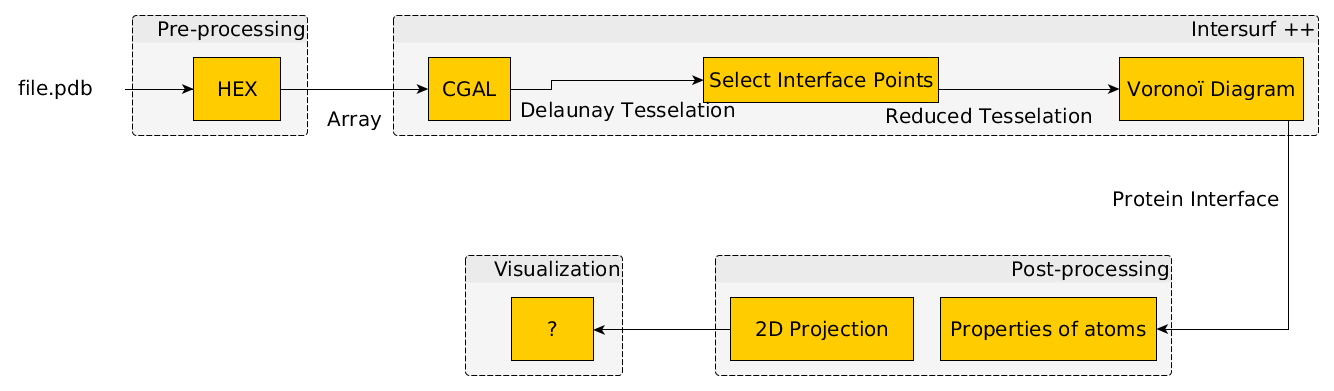
\includegraphics[width=\textwidth]{figures/flow_chart.png}
  \caption{Flow chart du programme}
  \label{fig::flow_chart}
\end{figure}

\section{Architecture Logicielle}
\begin{itemize}
  \item C / C++ / Libraries
  \item Compilation Cmake
\end{itemize}
Les différentes étapes


\section{Récupération de données + stockage}
\begin{itemize}
  \item .pdb files + pdb reader
  \item Tableau et méthode de stockage (C++ structures)
  \item CGAL structures : Delaunay + Polyhedron
\end{itemize}

Le point de départ du projet est de lire un fichier \textit{.pdb} et de le stocker
de manière à créer les structures fournies par CGAL. Nous avons utilisé une partie du programme
\textbf{Hex} développé en C par David Ritchie qui permet de \textit{parser} le fichier
\textit{.pdb} pour récupérer les données utiles du complexe étudié. Ces informations constituent
la référence utilisée lors de la construction de l'interface lorsque des détails
sur les atomes (chaîne, etc.) doivent êre connus. La fonction utilisée pour cela
renvoie un pointeur vers un tableau recensant toutes les informations utiles, c'est-à-dire
une image du fichier \textit{.pdb} que nous appellerons \textit{Image pdb} (voir
figure \ref{fig::read_pdb}).

\begin{figure}[ht]
\centering
  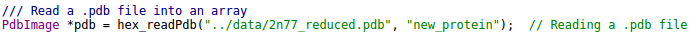
\includegraphics[width=\textwidth]{figures/pdb_image.png}
  \caption{Récupération des données du fichier \textit{.pdb}}
  \label{fig::read_pdb}
\end{figure}

Pour créer une structure de Delaunay, CGAL prend normalement une liste de points stockée
sous forme de tableau. Cependant, utiliser cette méthode simple ne premettrait pas d'accéder aux
informations contenues dans le fichier \textit{.pdb}. En effet, chaque vertice (point), de la
triangulation de Delaunay doit être indexé de manière à retrouver les informations voulues dans la
liste d'atome fournie par le fichier de départ. Les index doivent donc être choisis
au moment de la lecture de l'\textit{Image pdb} pour correspondre à la place de l'atome
dans le tableau.
Il existe deux méthodes pour insérer un index à une variable de type Vertex dans CGAL :
\begin{itemize}
  \item on modifie la classe Vertex en ajoutant un attribut
  \item on utilise une classe différente fournie par CGAL
\end{itemize}
Nous avons choisi d'utiliser la seconde méthode (voir figure \ref{fig::vertex_base}) pour
sa simplicité. Lors de l'instanciation, cette classe prend notamment en paramètre
\textit{template} un type qui de variable qui sera accessible comme l'attribut \textit{info()}.

\begin{figure}[ht]
\centering
  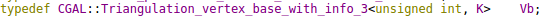
\includegraphics[width=0.8\textwidth]{figures/vertex_base.png}
  \caption{Déclaration de la classe \textit{Vertex\_base\_with\_info}}
  \label{fig::vertex_base}
\end{figure}

Le type de l'index est donc un entier positif qui fera partie de la structure Delaunay
et sera accessible lors du parcours de ces structures. Cependant, la structure de Delaunay
requiert l'ajout d'un index lors de son instanciation. Un vecteur de paires contenant
un point 3D et une variable du type de l'attribut \textit{info()} (voir figure
\ref{fig::vector_atom_index}) convient.

\begin{figure}[ht]
\centering
  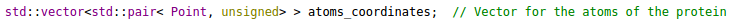
\includegraphics[width=\textwidth]{figures/vector_atom_index.png}
  \caption{Déclaration du vecteur contenant les atomes et leurs index}
  \label{fig::vector_atom_index}
\end{figure}

La fonction complète permettant d'écrire un fichier\textit{.pdb} dans une structure
\textit{CGAL::Delaunay} est disponible en annexe (voir figure \ref{fig::read_pdb}).
On remarque la présence de la \textit{map} C++ \textit{is\_interface}
(voir figure \ref{fig::is_interface}) qui sera utilisée par la suite
pour sélectionner les tétrahèdres présents à l'interface (voir figure \ref{fig::delaunays}).

\begin{figure}[ht]
\centering
  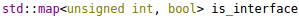
\includegraphics[width=0.5\textwidth]{figures/is_interface.png}
  \caption{Déclaration de la map is\_interface}
  \label{fig::is_interface}
\end{figure}

\section{Construction de la surface}
\begin{itemize}
  \item Tesselation $\to$ Arêtes à l'interface $\to$ Dual (Surface)
  \item Index + Informations : Lien entre le .pdb (Chaîne, Atome, etc.) et les points de la surface
  \item smoothing
\end{itemize}



\section{Affichage}
\begin{itemize}
  \item .off files $\to$ écriture avec indexation
\end{itemize}

Pour l'affichage des protéines et de l'interface, nous avons choisi les fichiers
\textit{.off} qui permettent de stocker une liste de points (colorés ou non) et
d'indiquer les liens entre chacun de ces points (voir figure \ref{fig::off_file}).

\begin{figure}[ht]
\centering
  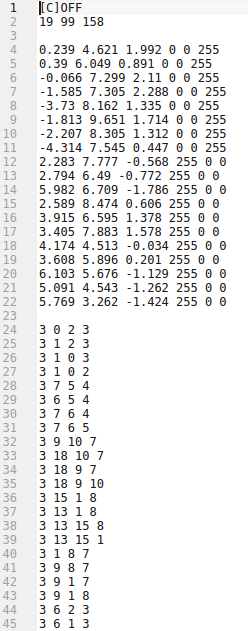
\includegraphics[width=0.3\textwidth]{figures/off_file.png}
  \caption{Exemple de fichier \textit{.off}}
  \label{fig::off_file}
\end{figure}

La première ligne indique le type de fichier (OFF) et la présence ou non de coloration :
[C] si oui un espace vide sinon. La seconde ligne donne, dans cet ordre, le nombre
de points, le nombre de cellules (polyhèdres) et le nombre d'arêtes ce dernier n'étant
pas nécessaire à la lecture du fichier. Dans notre exemple, les lignes 4 à 22 listent
les coordonnées des points et la couleur associée à chacun. La couleur est stockée en RGB
(Rouge, Vert, Bleu) avec des entiers entre 0 et 255 ou des flottants entre 0.0 et 1.0.

Au delà de la ligne 23, les cellules sont listées, avec comme premier entier à chaque
ligne, le nombre de points de la cellule. Comme notre exemple représente une triangulation
de Delaunay, ce nombre vaut 3 car chaque face de la triangulation correspond à un
triangle. A la suite de cet entier viennent les indices des points composant la cellule
(ou la face). Cet indice correspond à la place des coordonnées listées plus haut.
